%
%
% -------------------------------------------------
%
\documentclass[11pt, a4paper]{amsart}
%
%
%
\usepackage[latin1]{inputenc}
\usepackage[english]{babel}
\selectlanguage{english}
%
\usepackage{hyperref}
\usepackage[twoside=false]{geometry}
% \usepackage{cmbright}
\usepackage{bm}
\usepackage{cleveref}
\usepackage{xparse}
\usepackage[textsize=footnotesize]{todonotes}
\usepackage{subfigure}
\usepackage{float}
%
%
%
\title{Sensor Fusion Final Project}
\author{Hans Franzen}
\date{}
%
%
% ----------------------------------------------------------------------------------------------------
%
%
\begin{document}

	\maketitle
	
	The tracking exercise consisted of four steps:
	\begin{enumerate}
		\item Implement an extended Kalman filter. This was done in the file \texttt{filter.py}. The state transition matrix $F$, the process noise covariance matrix $Q$, the residual $\gamma$ and the matrix $S$ were implemented, along with the prediction and update functions. The RMSE is in Figure \ref{RMSE1}.
		\begin{figure}
			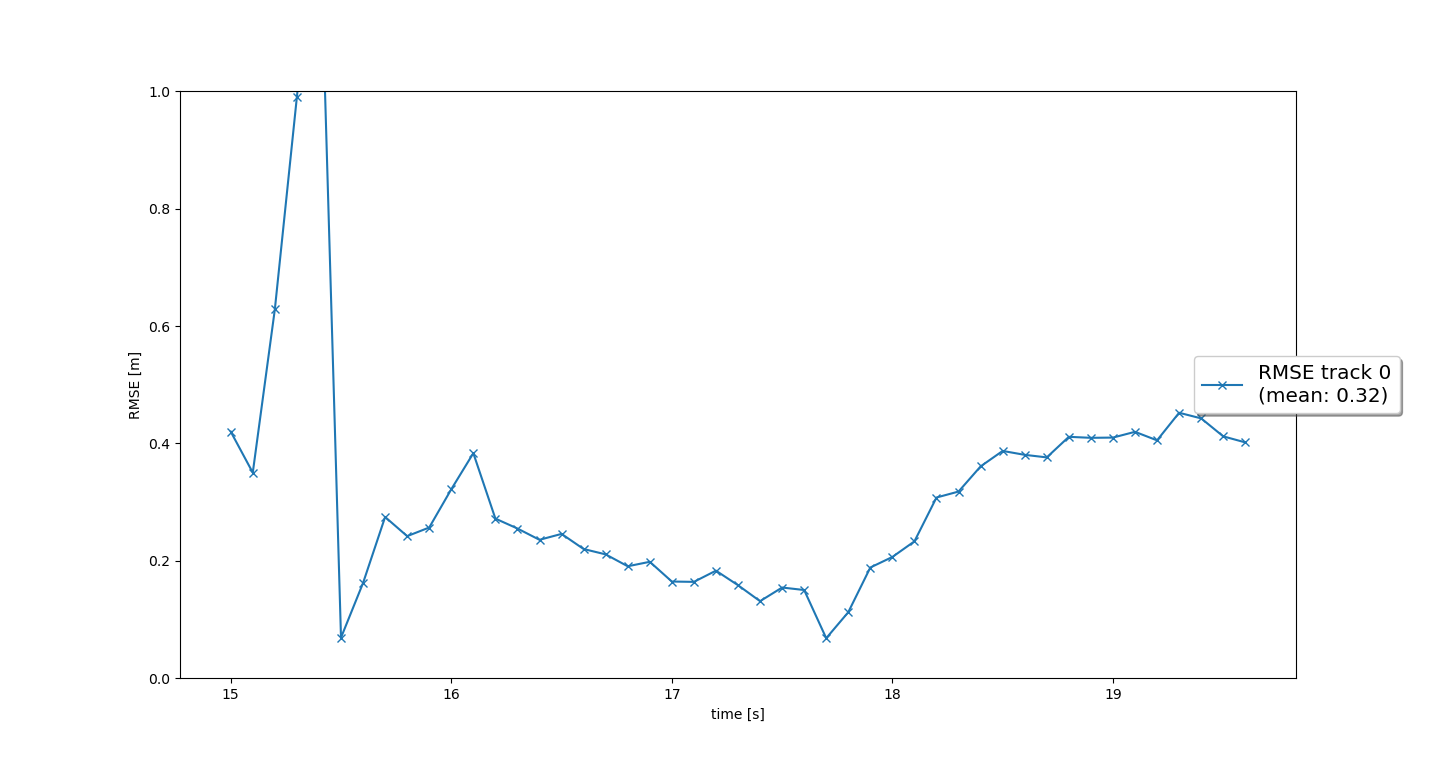
\includegraphics[scale=0.4]{../images_output/RMSE1.png}
			\caption{RMSE in Step 1}
			\label{RMSE1}
		\end{figure}
		%
		\item Manage tracks. The respective code can be found in \texttt{trackmanagement.py}. New tracks are being initialized, a track score is maintained, a track status (initialized, tentative, confirmed) is set and updated, and tracks are being deleted once the track score drops below a threshold or the positional uncertainty is too big. The RMSE can be found in Figure \ref{RMSE2}.
		\begin{figure}
			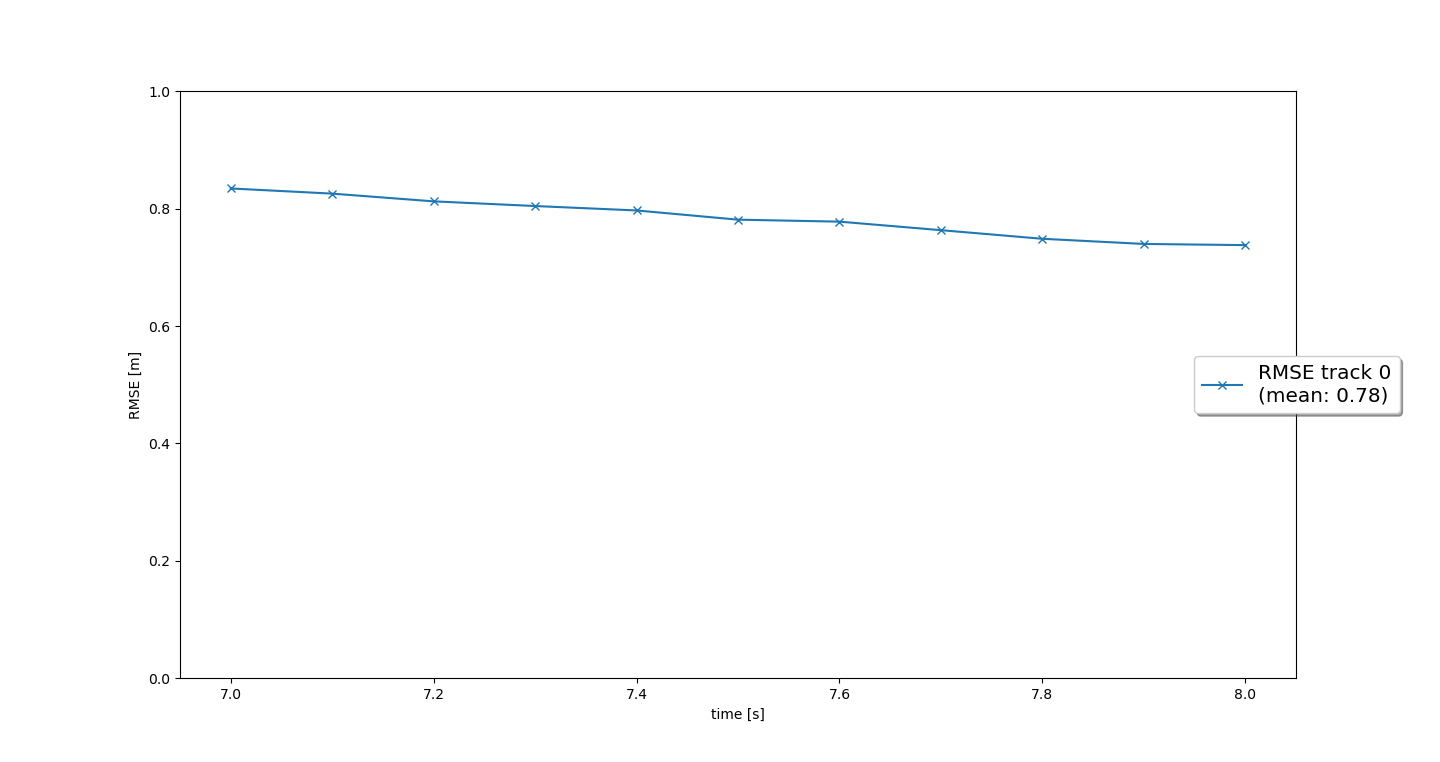
\includegraphics[scale=0.4]{../images_output/RMSE2.png}
			\caption{RMSE in Step 2}
			\label{RMSE2}
		\end{figure}
		%
		\item Associate tracks to measurements. This happens in the file \texttt{association.py}. The Mahalanobis distance between a track and a measurement is computed and an association matrix is set up accordingly. A gating threshold is applied. Then an association is made using the simple nearest neighbor algorithm. The RMSE is depicted in Figure \ref{RMSE3}.
		\begin{figure}
			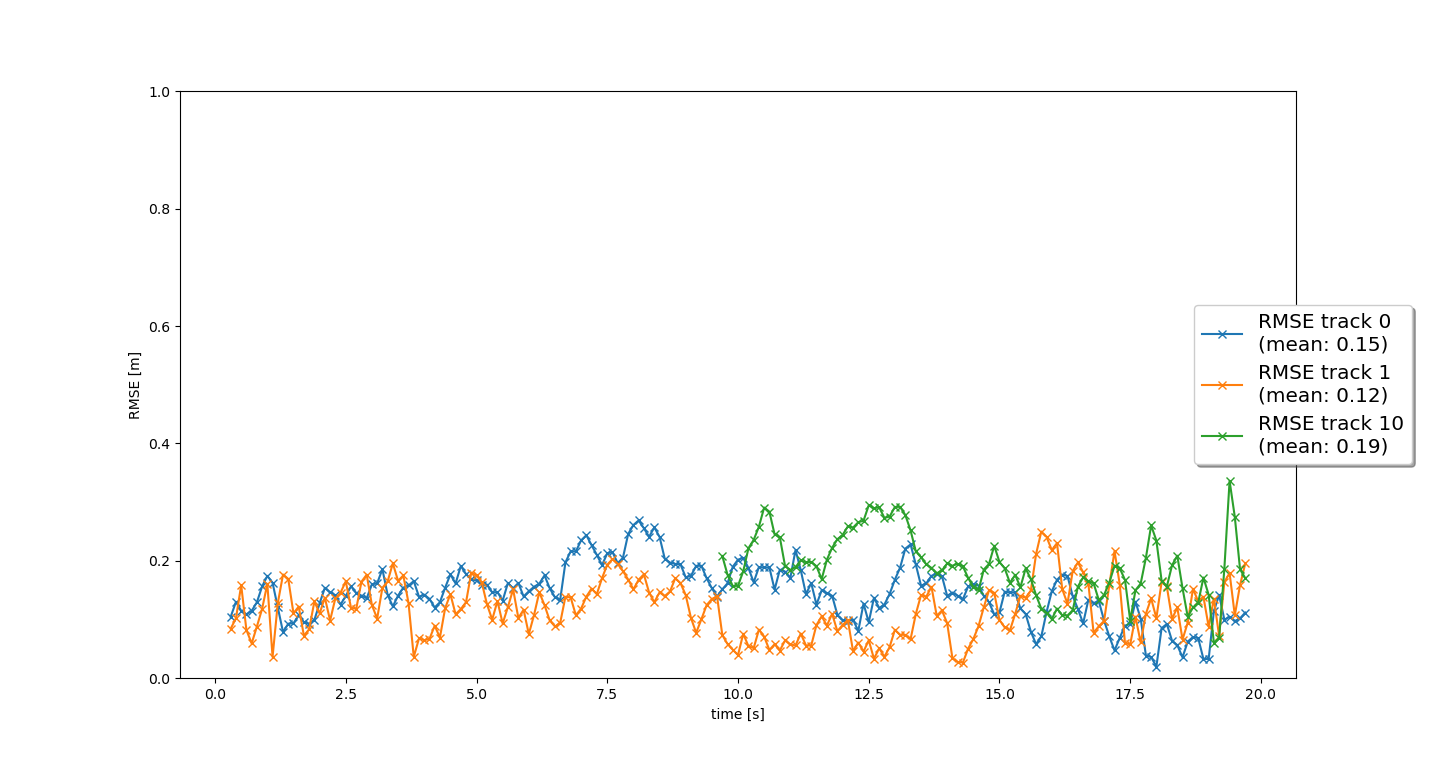
\includegraphics[scale=0.4]{../images_output/RMSE3.png}
			\caption{RMSE in Step 3}
			\label{RMSE3}
		\end{figure}
		%
		\item Fusion with camera sensors. This is done in \texttt{measurements.py}. While the above three steps only included lidar measurements, we now use camera measurements as well. We implement their field of view, the measurement function $h$ and initialize new measurements. The RMSE is as shown in Figure \ref{RMSE4}.
		\begin{figure}
			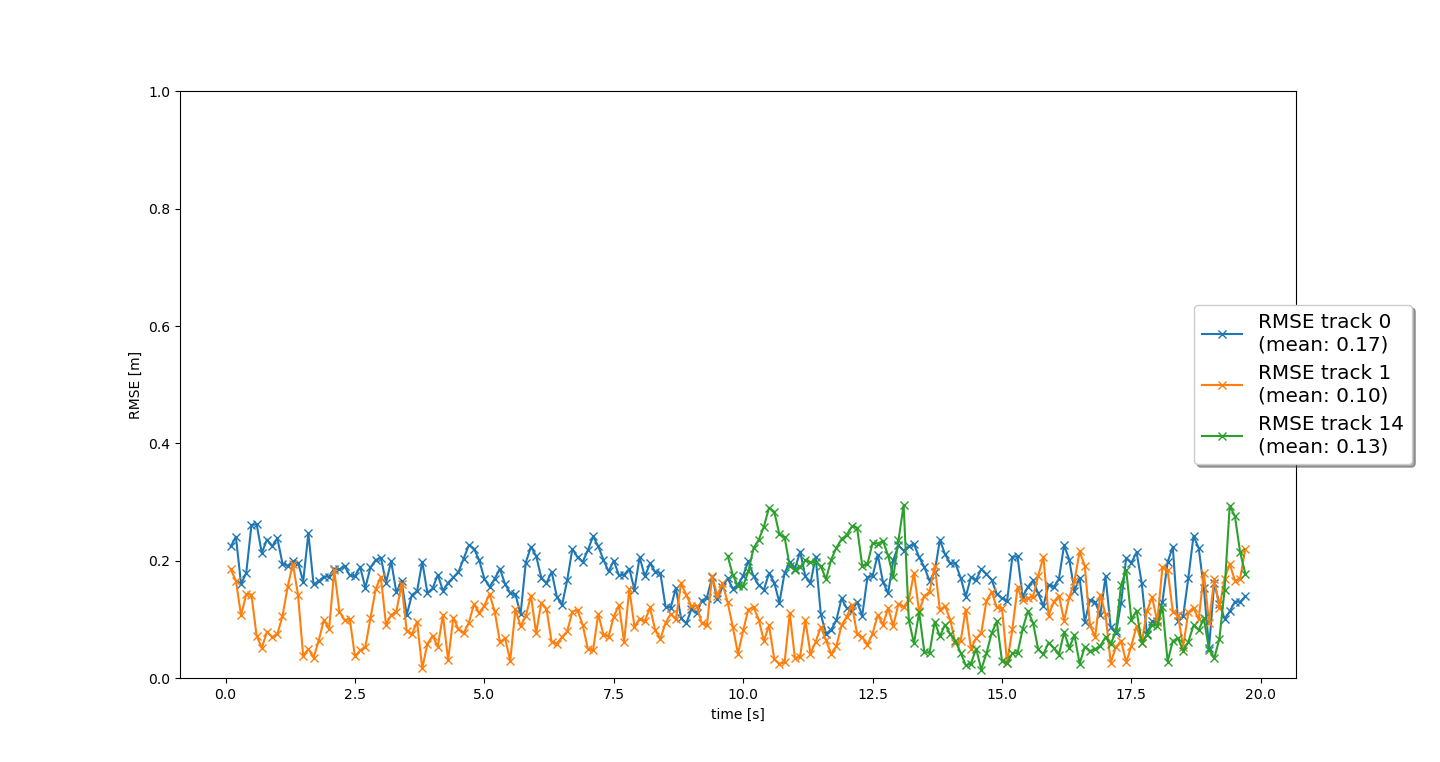
\includegraphics[scale=0.4]{../images_output/RMSE4.png}
			\caption{RMSE in Step 4}
			\label{RMSE4}
		\end{figure}
	\end{enumerate}
	
	The step which took most time for me was Step 4. I had a typo in initialization which resulted in very strange results. Due to the many function calls it was very difficult to debug.
	
	Using both camera and lidar measurements had a significant effect on the performance of tracking. Ghost tracks which appeared in the lidar-only tracking in Step 3 disappeared much faster with camera measurements. Also, the RMSE tends to be lower, although just a bit.
	
	Challenges for tracking in real-life scenarios are, e.g., the limitations of the respective sensors (the data for the project was taken on a clear day, which isn't always the case) and a trade-off between model complexity and computational performance. The more complex a model is, the better the results can be but also the more costly the computations become.
	
	The results can be improved by, e.g., using a non-linear model, improving the association algorithm (global nearest neighbor or JPDA), or simply adding more sensors.

\end{document}
